\documentclass[tikz,border=5pt]{standalone}
\usepackage{tikz}
\usetikzlibrary{positioning,arrows.meta,shapes.multipart,fit}

\begin{document}

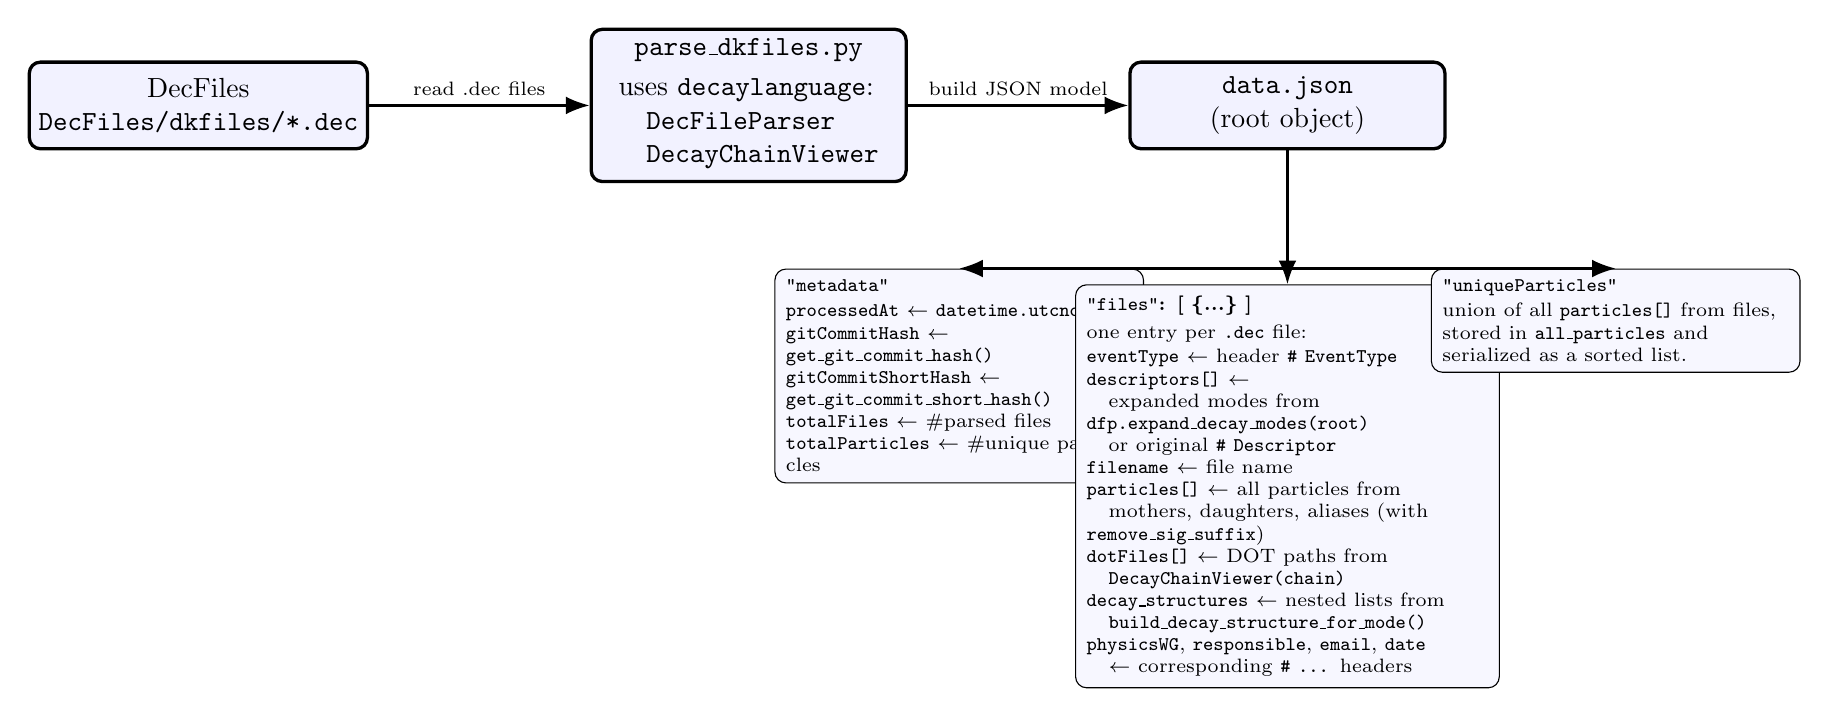
\begin{tikzpicture}[
  node distance=1.8cm and 2.8cm,
  box/.style={rectangle, rounded corners, draw=black, very thick, fill=blue!5, align=center, minimum width=4.0cm, minimum height=1.1cm},
  smallbox/.style={rectangle, rounded corners, draw=black, fill=blue!3, align=left, font=\scriptsize, inner sep=4pt},
  arrow/.style={-{Latex[length=3mm]}, thick},
  label/.style={font=\scriptsize}
]

% Left: input DecFiles
\node[box] (decfiles) {DecFiles\\\texttt{DecFiles/dkfiles/*.dec}};

% Parser core
\node[box, right=of decfiles] (parser) {\texttt{parse\_dkfiles.py}\\[3pt]
  \begin{tabular}{@{}l@{}}
    uses \texttt{decaylanguage}:\\
    \quad \texttt{DecFileParser}\\
    \quad \texttt{DecayChainViewer}
  \end{tabular}
};

% JSON root object
\node[box, right=of parser] (jsonroot) {\texttt{data.json}\\(root object)};

% Arrows main pipeline
\draw[arrow] (decfiles) -- node[above,label]{read .dec files} (parser);
\draw[arrow] (parser) -- node[above,label]{build JSON model} (jsonroot);

% Three-column breakdown of fields
\node[smallbox, below left=1.5cm and -0.2cm of jsonroot, text width=4.4cm] (meta) {
  \textbf{\texttt{"metadata"}}\\[1pt]
  \texttt{processedAt} $\leftarrow$ \texttt{datetime.utcnow()}\\
  \texttt{gitCommitHash} $\leftarrow$ \texttt{get\_git\_commit\_hash()}\\
  \texttt{gitCommitShortHash} $\leftarrow$ \texttt{get\_git\_commit\_short\_hash()}\\
  \texttt{totalFiles} $\leftarrow$ \#parsed files\\
  \texttt{totalParticles} $\leftarrow$ \#unique particles
};

\node[smallbox, below=1.7cm of jsonroot, text width=5.1cm] (files) {
  \textbf{\texttt{"files"}: [ \{...\} ]}\\[2pt]
  one entry per \texttt{.dec} file:\\[1pt]
  \texttt{eventType} $\leftarrow$ header \texttt{\# EventType}\\
  \texttt{descriptors[]} $\leftarrow$\\
  \quad expanded modes from \texttt{dfp.expand\_decay\_modes(root)}\\
  \quad or original \texttt{\# Descriptor}\\
  \texttt{filename} $\leftarrow$ file name\\
  \texttt{particles[]} $\leftarrow$ all particles from\\
  \quad mothers, daughters, aliases (with \texttt{remove\_sig\_suffix})\\
  \texttt{dotFiles[]} $\leftarrow$ DOT paths from\\
  \quad \texttt{DecayChainViewer(chain)}\\
  \texttt{decay\_structures} $\leftarrow$ nested lists from\\
  \quad \texttt{build\_decay\_structure\_for\_mode()}\\
  \texttt{physicsWG}, \texttt{responsible}, \texttt{email}, \texttt{date}\\
  \quad $\leftarrow$ corresponding \texttt{\# ...} headers
};

\node[smallbox, below right=1.5cm and -0.2cm of jsonroot, text width=4.4cm] (upart) {
  \textbf{\texttt{"uniqueParticles"}}\\[1pt]
  union of all \texttt{particles[]} from files,\\
  stored in \texttt{all\_particles} and\\
  serialized as a sorted list.
};

% Connect root JSON box to field groups
\draw[arrow] (jsonroot.south) |- (meta.north);
\draw[arrow] (jsonroot.south) -- (files.north);
\draw[arrow] (jsonroot.south) |- (upart.north);

\end{tikzpicture}

\end{document}


